\chapter{Caracterización y puesta en servicio}

En este capitulo se expondran los procesos de caracterizacion y puesta en servicio del telescopio CPT. Para abordar los puntos de caracterizacion y primera luz de los objetivos propuestos para este trabajo. Se detallaran los aspectos considerados para cada una de las mediciones y los fundamentos correspondientes.

\section{Enfoque del alimentador}

Se relizaron 2 mediciones de enfoque del alimentador, una a 70 metros y otra a 186 metros. Para la primera medicion se utilizo un generador de senales generico con una LPDA de bajo ancho de banda. Luego para el resto de las mediciones se utilizo la estrella artificial de la copa de agua de la seccion XX.\\

\subsection{Alimentador sin soportes a 70 metros}

En principios el alimentador de telesecopio consistia en una antena LPDA (Log Periodic Dipole Array) de 296 MHz a 6 GHz, de ultra ancho de banda, con una ganancia de aproximadamente 9dBi. Con el receptor instalado en esta antena, se procedio a realizar el enfoque del alimentador. Para esta etapa se retiraro el soporte tetrapodo y se instalo el alimentador en un tripode auxiliar sostenido por un tubo de PVC para lograr la altura del centro del reflector de 2 metros.\\

\begin{figure}
    \centering
    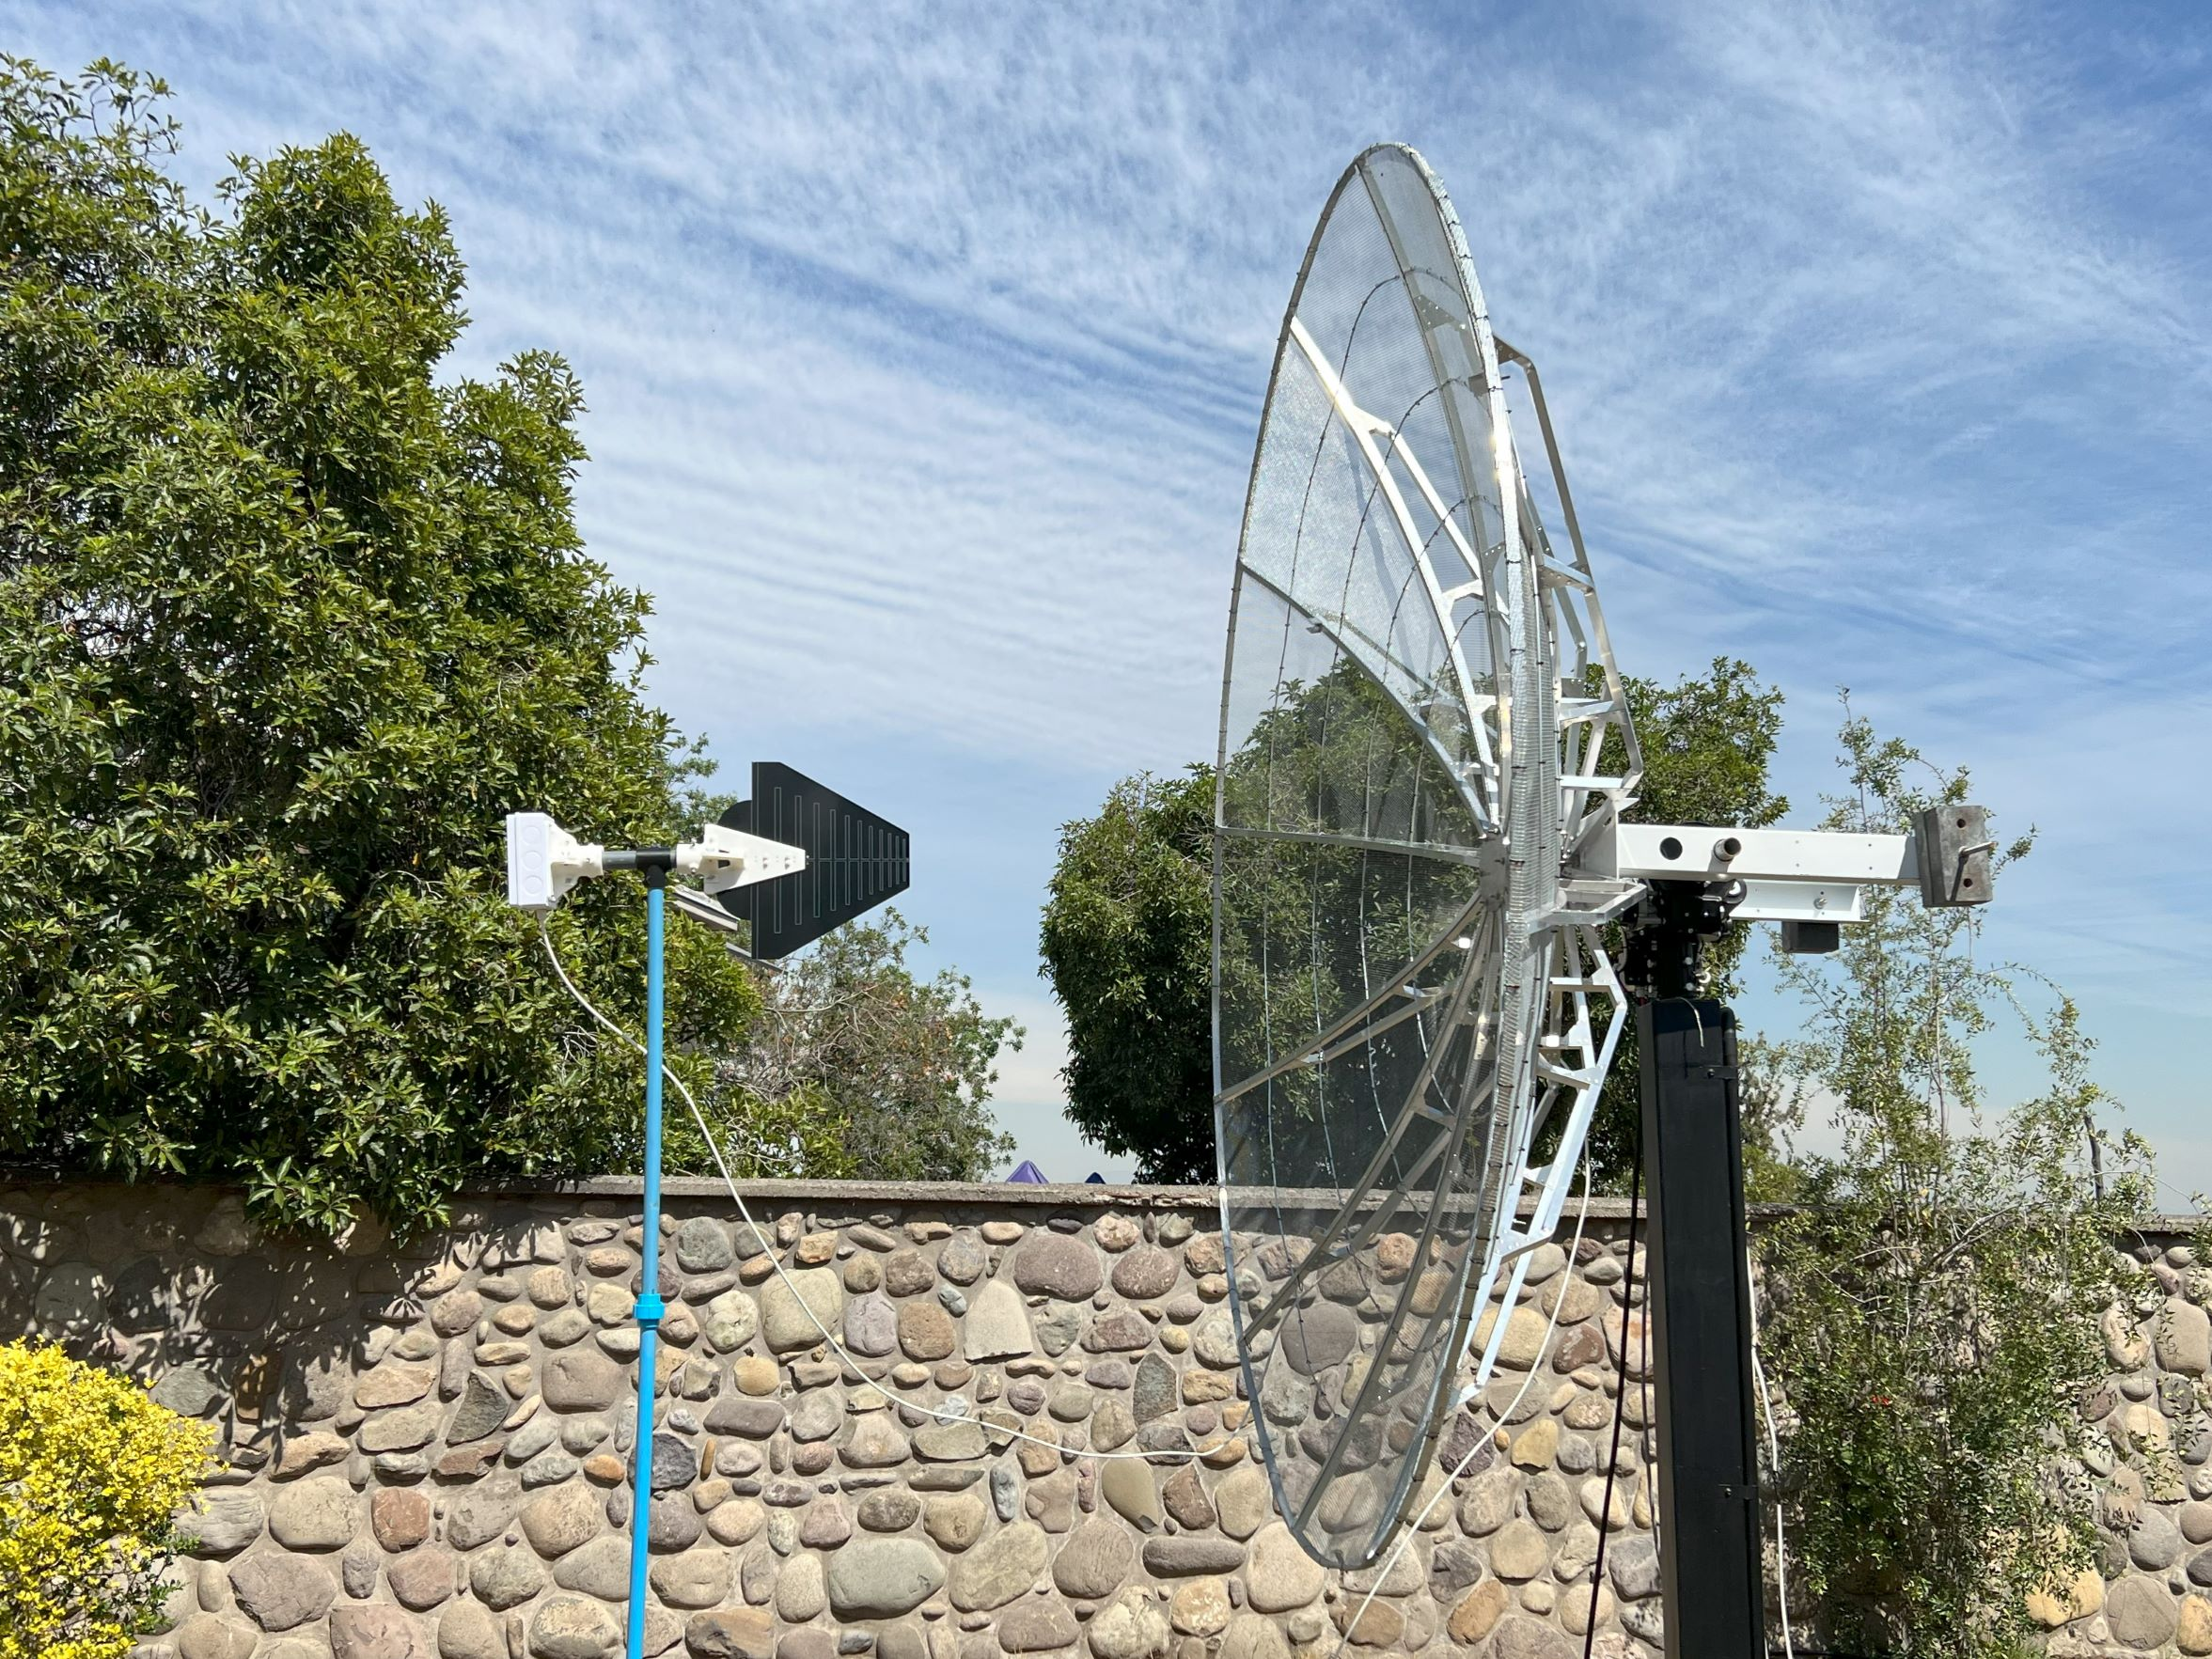
\includegraphics[width=0.7\textwidth]{img/enfoque1}
    \caption{Antena LPDA en tripode auxiliar a 2 metros de altura.}
    \label{fig:antena_lpda}
\end{figure}

Con la antena de la figura \ref{fig:antena_lpda} se procedio a realizar el enfoque del alimentador. La medicion consiste en mover el alimentador en el eje Z, es decir en la direccion de la apertura del reflector. A una distancia de 70 metros desde el relfector se instaló sobre otro tripode un generador de señales portatil con otra LPDA de menor ancho de banda.\\

\begin{figure}[h!]
    \centering
    \begin{subfigure}{0.45\textwidth}
        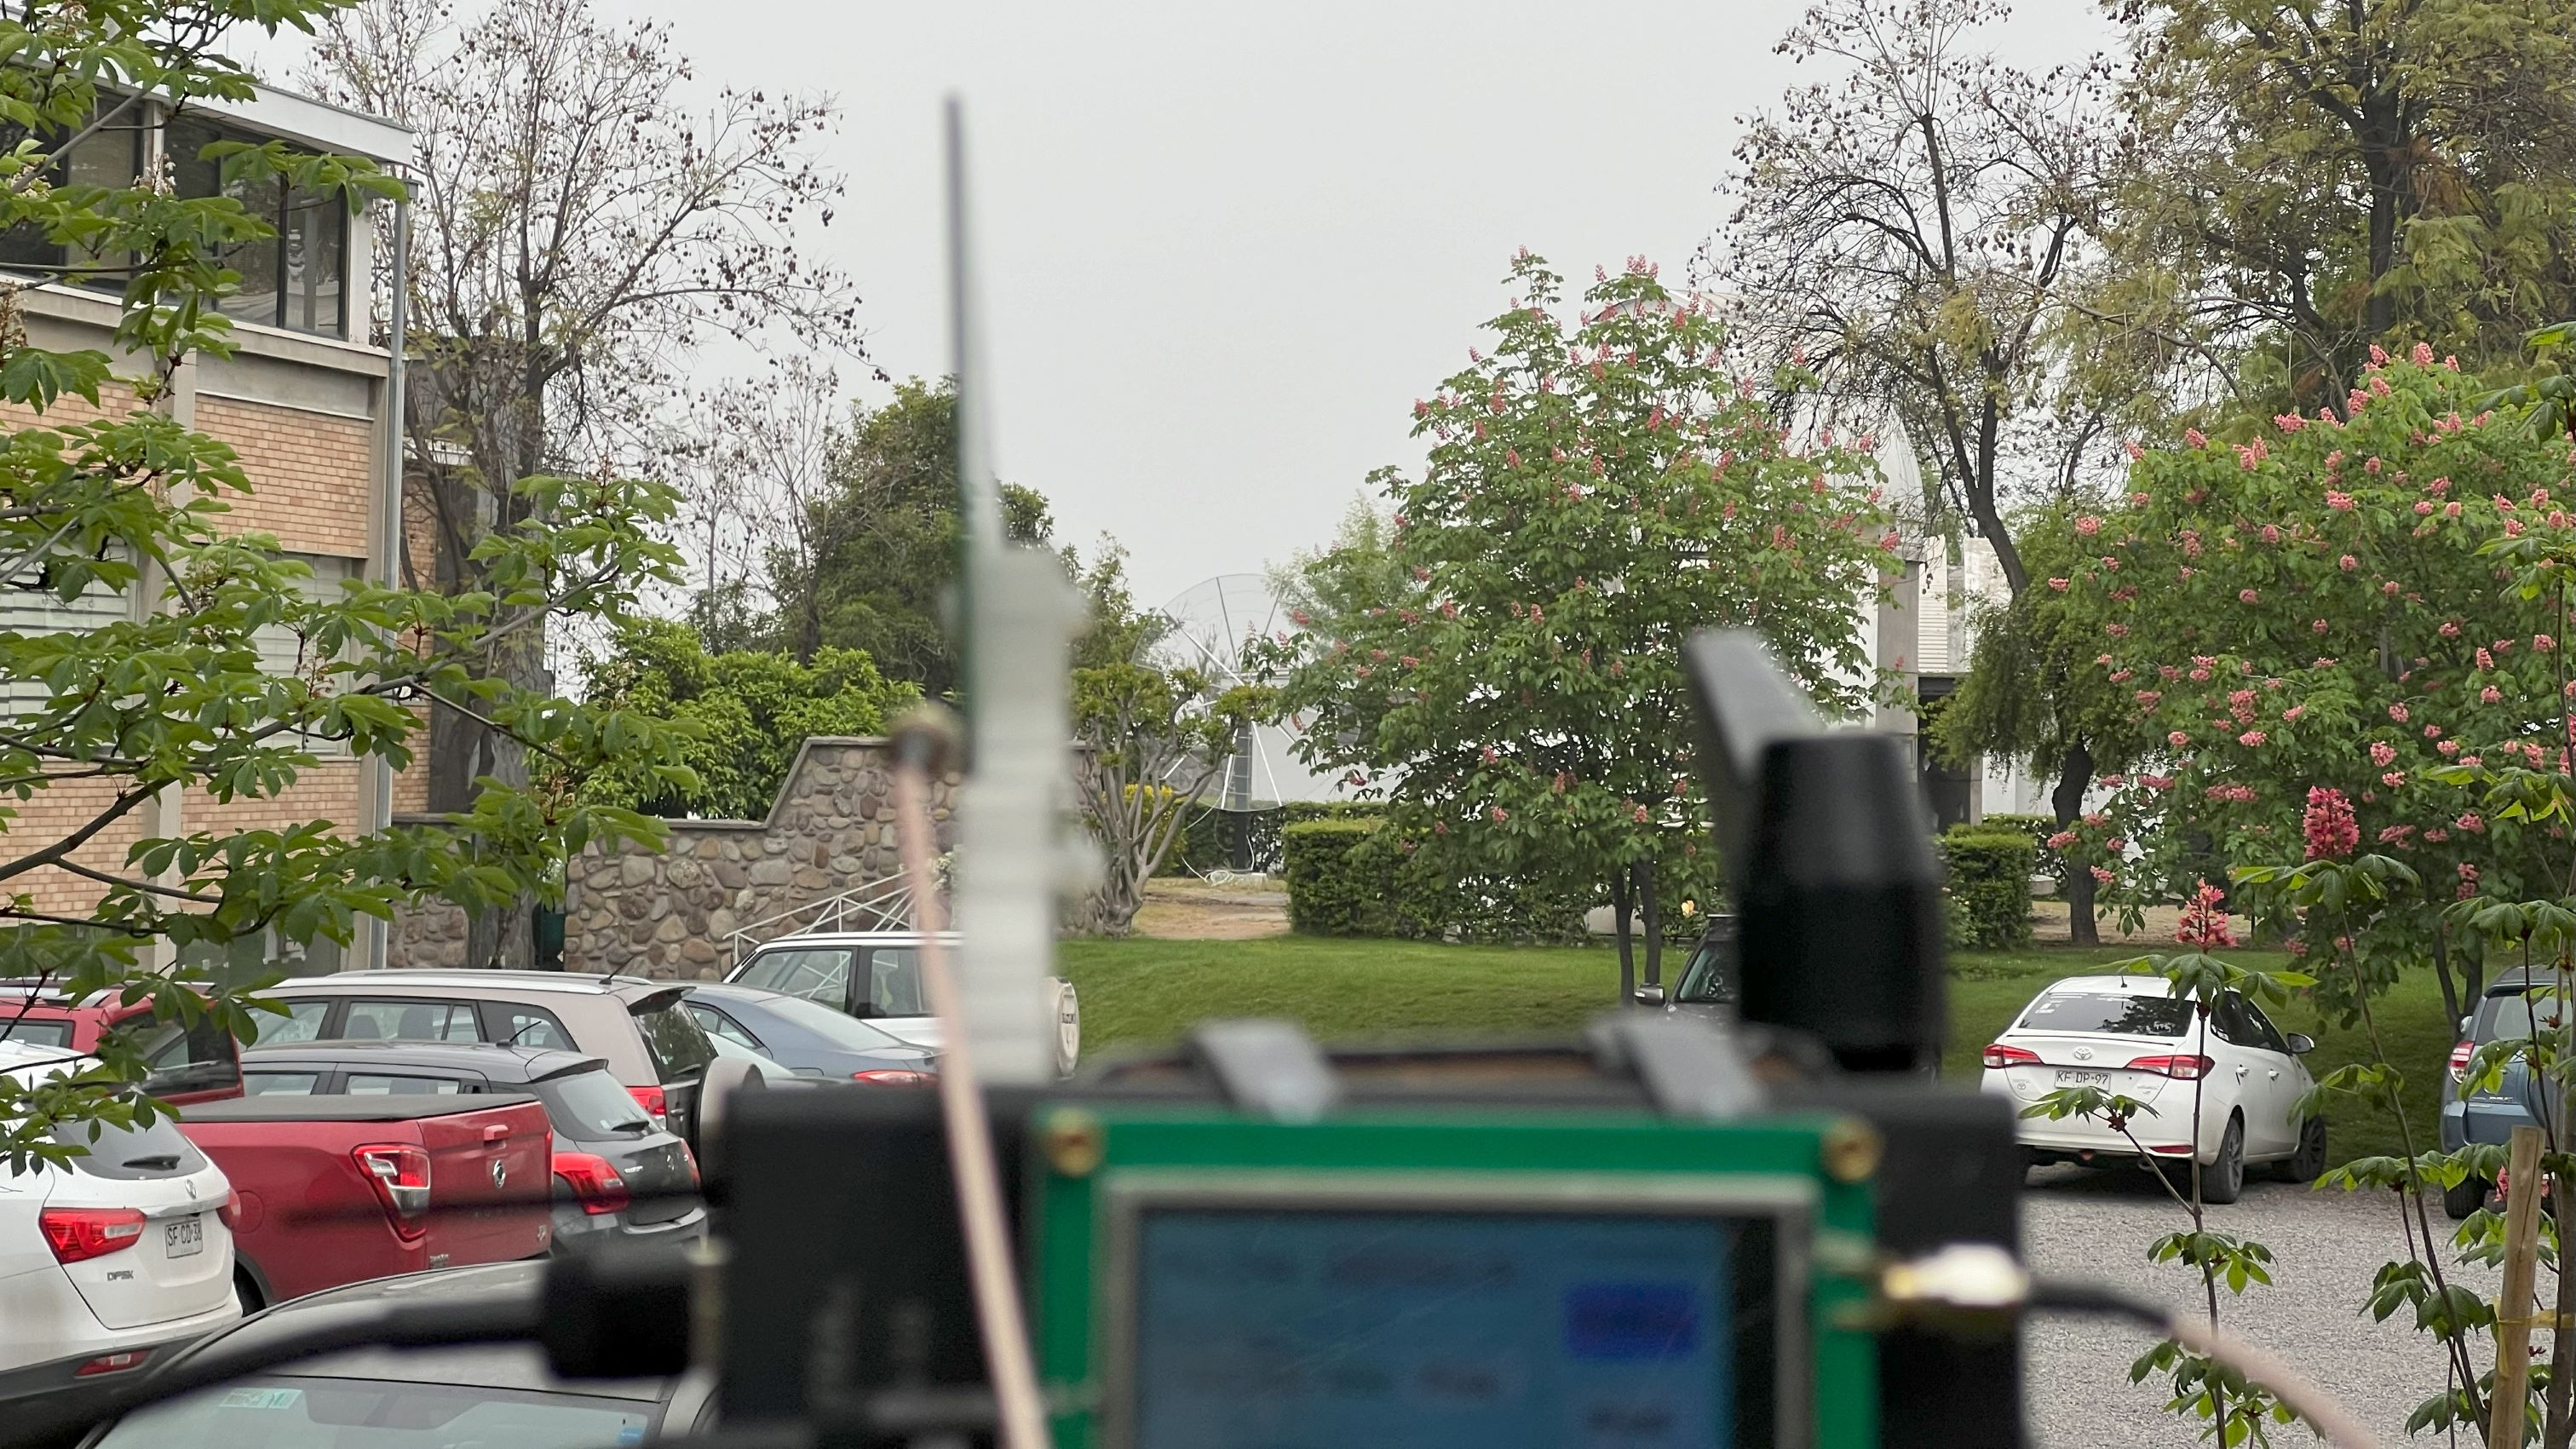
\includegraphics[width=\textwidth]{img/enfoque_cerca}
        \caption{Generador de señales portatil con la antena orientada hacia el reflector a 70 metros.}
        \label{fig:generador}
    \end{subfigure}
    \begin{subfigure}{0.45\textwidth}
        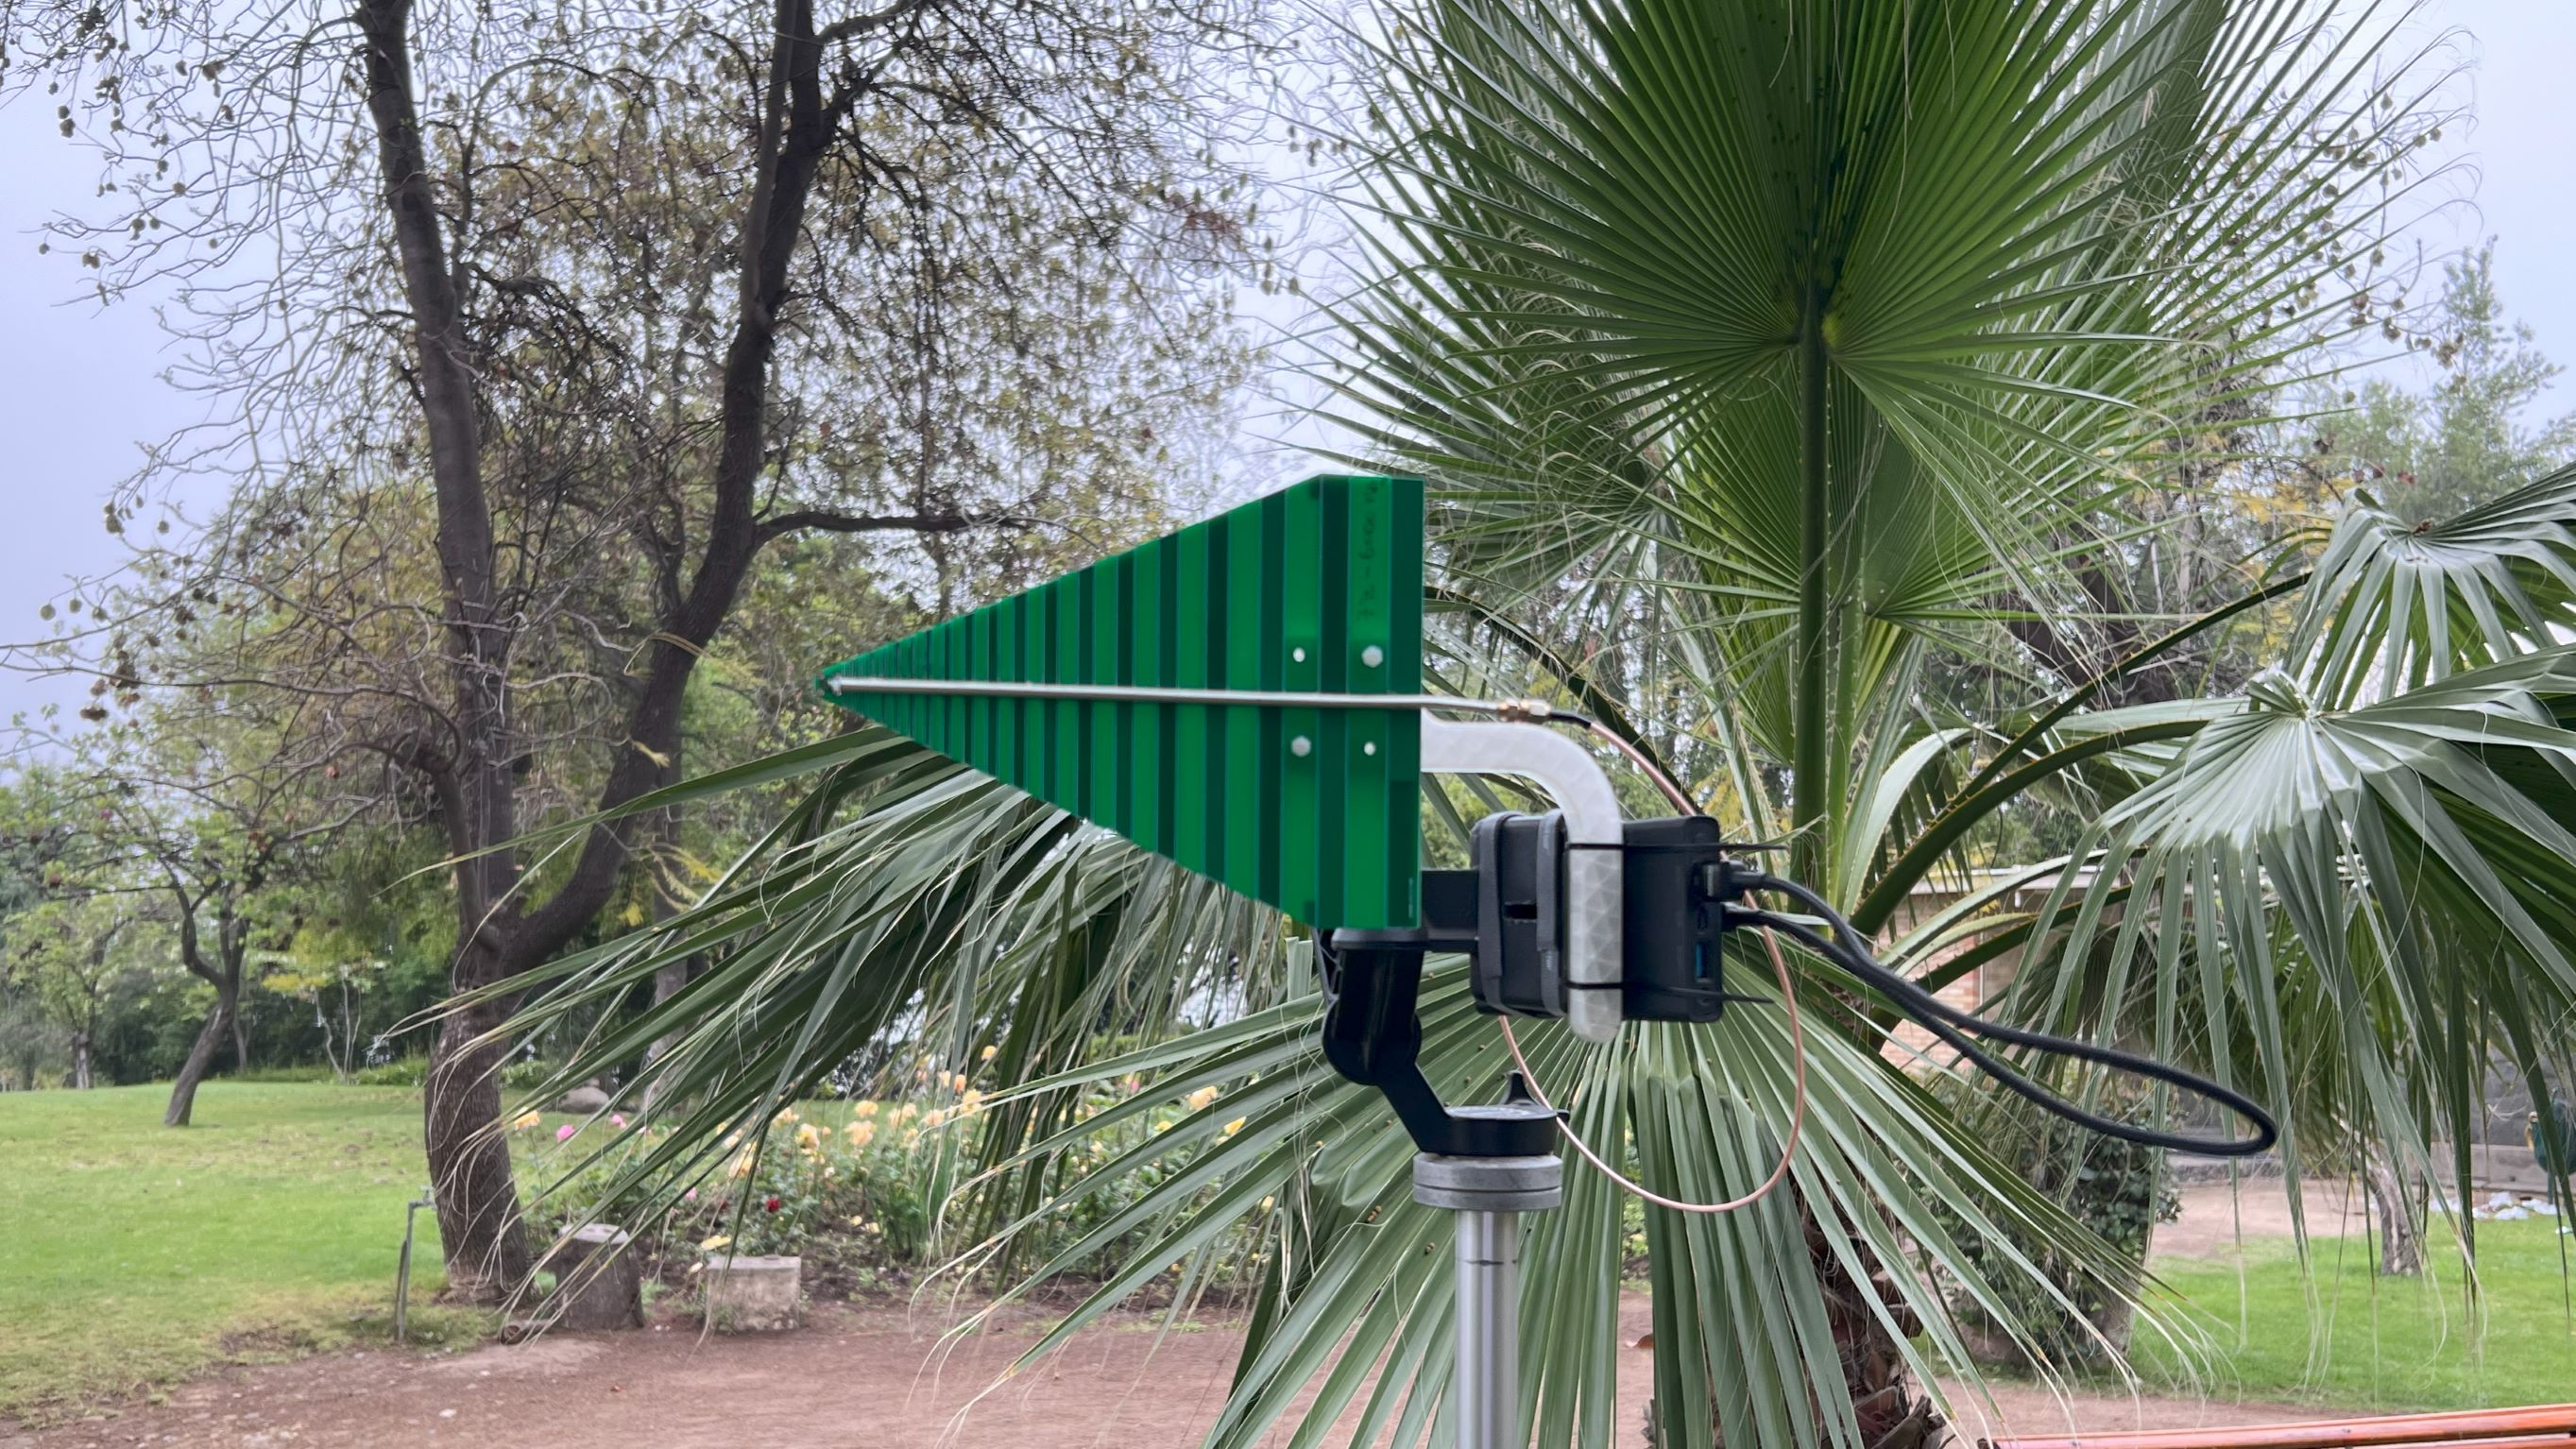
\includegraphics[width=\textwidth]{img/enfoque_cerca1}
        \caption{Antena LPDA de menor ancho de banda instalada con el generador de señales en tripode.}
        \label{fig:antena_lpda}
    \end{subfigure}
\end{figure}

El generador de señales se configuro a una frecuencia de 1000MHz y se disparo constantemente el tono en dicha frecuencia. Se instalo a una distancia de 70 metros dentro del praque cerro Calan con la consideracion que por la apertura de 3 metros del reflector se obtiene un campo lejano de 60.5 metros a 1000MHz, por lo que este generador se encontraba en el campo lejano del reflector.\\

\begin{figure}
    \centering
    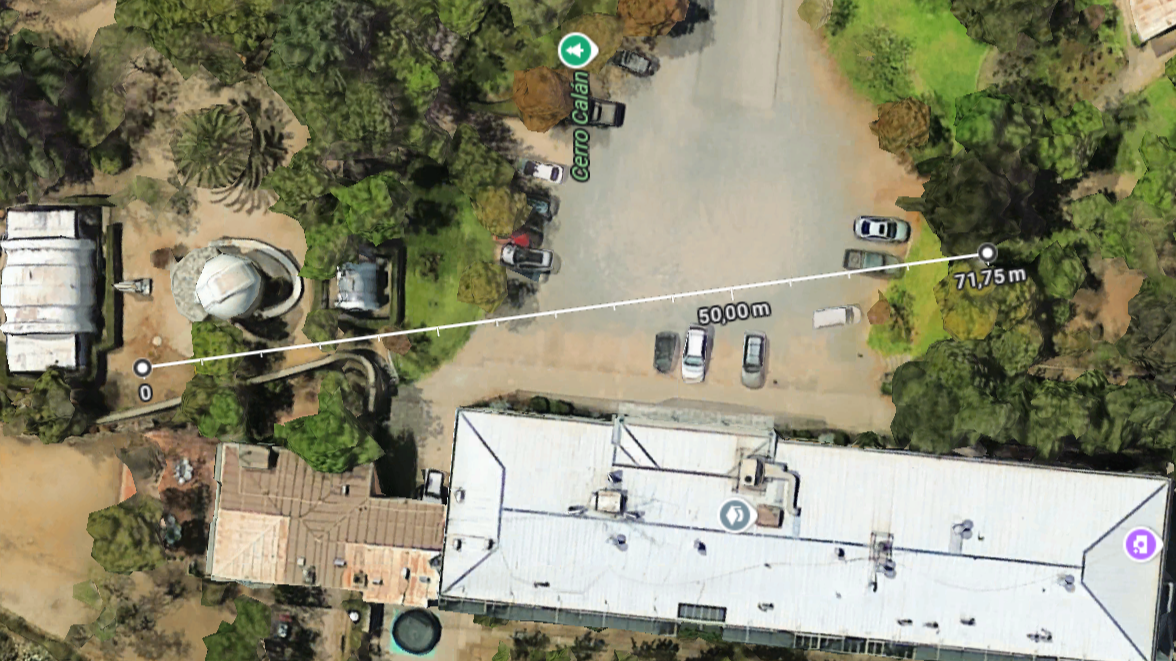
\includegraphics[width=0.7\textwidth]{img/70m_measure}
    \caption{Distancia de 70 metros entre el reflector y el generador de señales con elevaciones similares.}
    \label{fig:70m_measure}
\end{figure} 

En la figura \ref{fig:70m_measure} se muestra la distancia aproximada de 70 metros, tomando 10 metros de distancia adicional para asegurar el campo lejano a dicha frecuencia. Se alineo visualmente la antena del generador con el reflector a la distancia, la que se encuentra parcialemente con una linea de vista obstaculisada por arboles y arbustos.\\

Para efectos de la medicion, como se quiere encontrar un punto aproximado de enfoque la exactitud de esta medicion no es critica. Se procedio a mover el alimentador en el eje Z, es decir en la direccion de la apertura del reflector, hasta encontrar el punto donde la señal del generador era maxima.\\

La potencia recibida por el receptor fue medida con el software de medicon utilizando la RTL-SDR guardando los espectros para distancias de 5 cm en 5 cm. Se midio la razon señal a ruido y se obtuvo el punto de maxima potencia recibida en dBFS. Medidas que luego son calibradas en dBm por la medicion de sensibilidad.\\

\subsection{Alimentador con soportes con la estrella artificial}

Para la medicion de enfoque con la estrella artificial se instalo el soporte tetrapodo y se coloco el alimentador en su posicion final despues de las mediciones anteriores. Se configuro generador de señales valon de la estrella artificial a 1428MHz. Se utiliza esta nueva frecuencia para evitar interferencia de radio frecuencia en la medicion, utilziando el filtro delgado de H1.\\

Para el caso de 1428MHz, la distancia de campo lejano es de 85 metros y la estrella artificial se encuentra a 186 metros, estando perfectamente en el campo lejano del reflector. Ademas la alineacion con el reflector se realzia con el control automatico de la montura alt azimutal y la liena de vista se encuentra completamente libre para la priemra zona de fresnel.\\

\begin{figure}
    \centering
    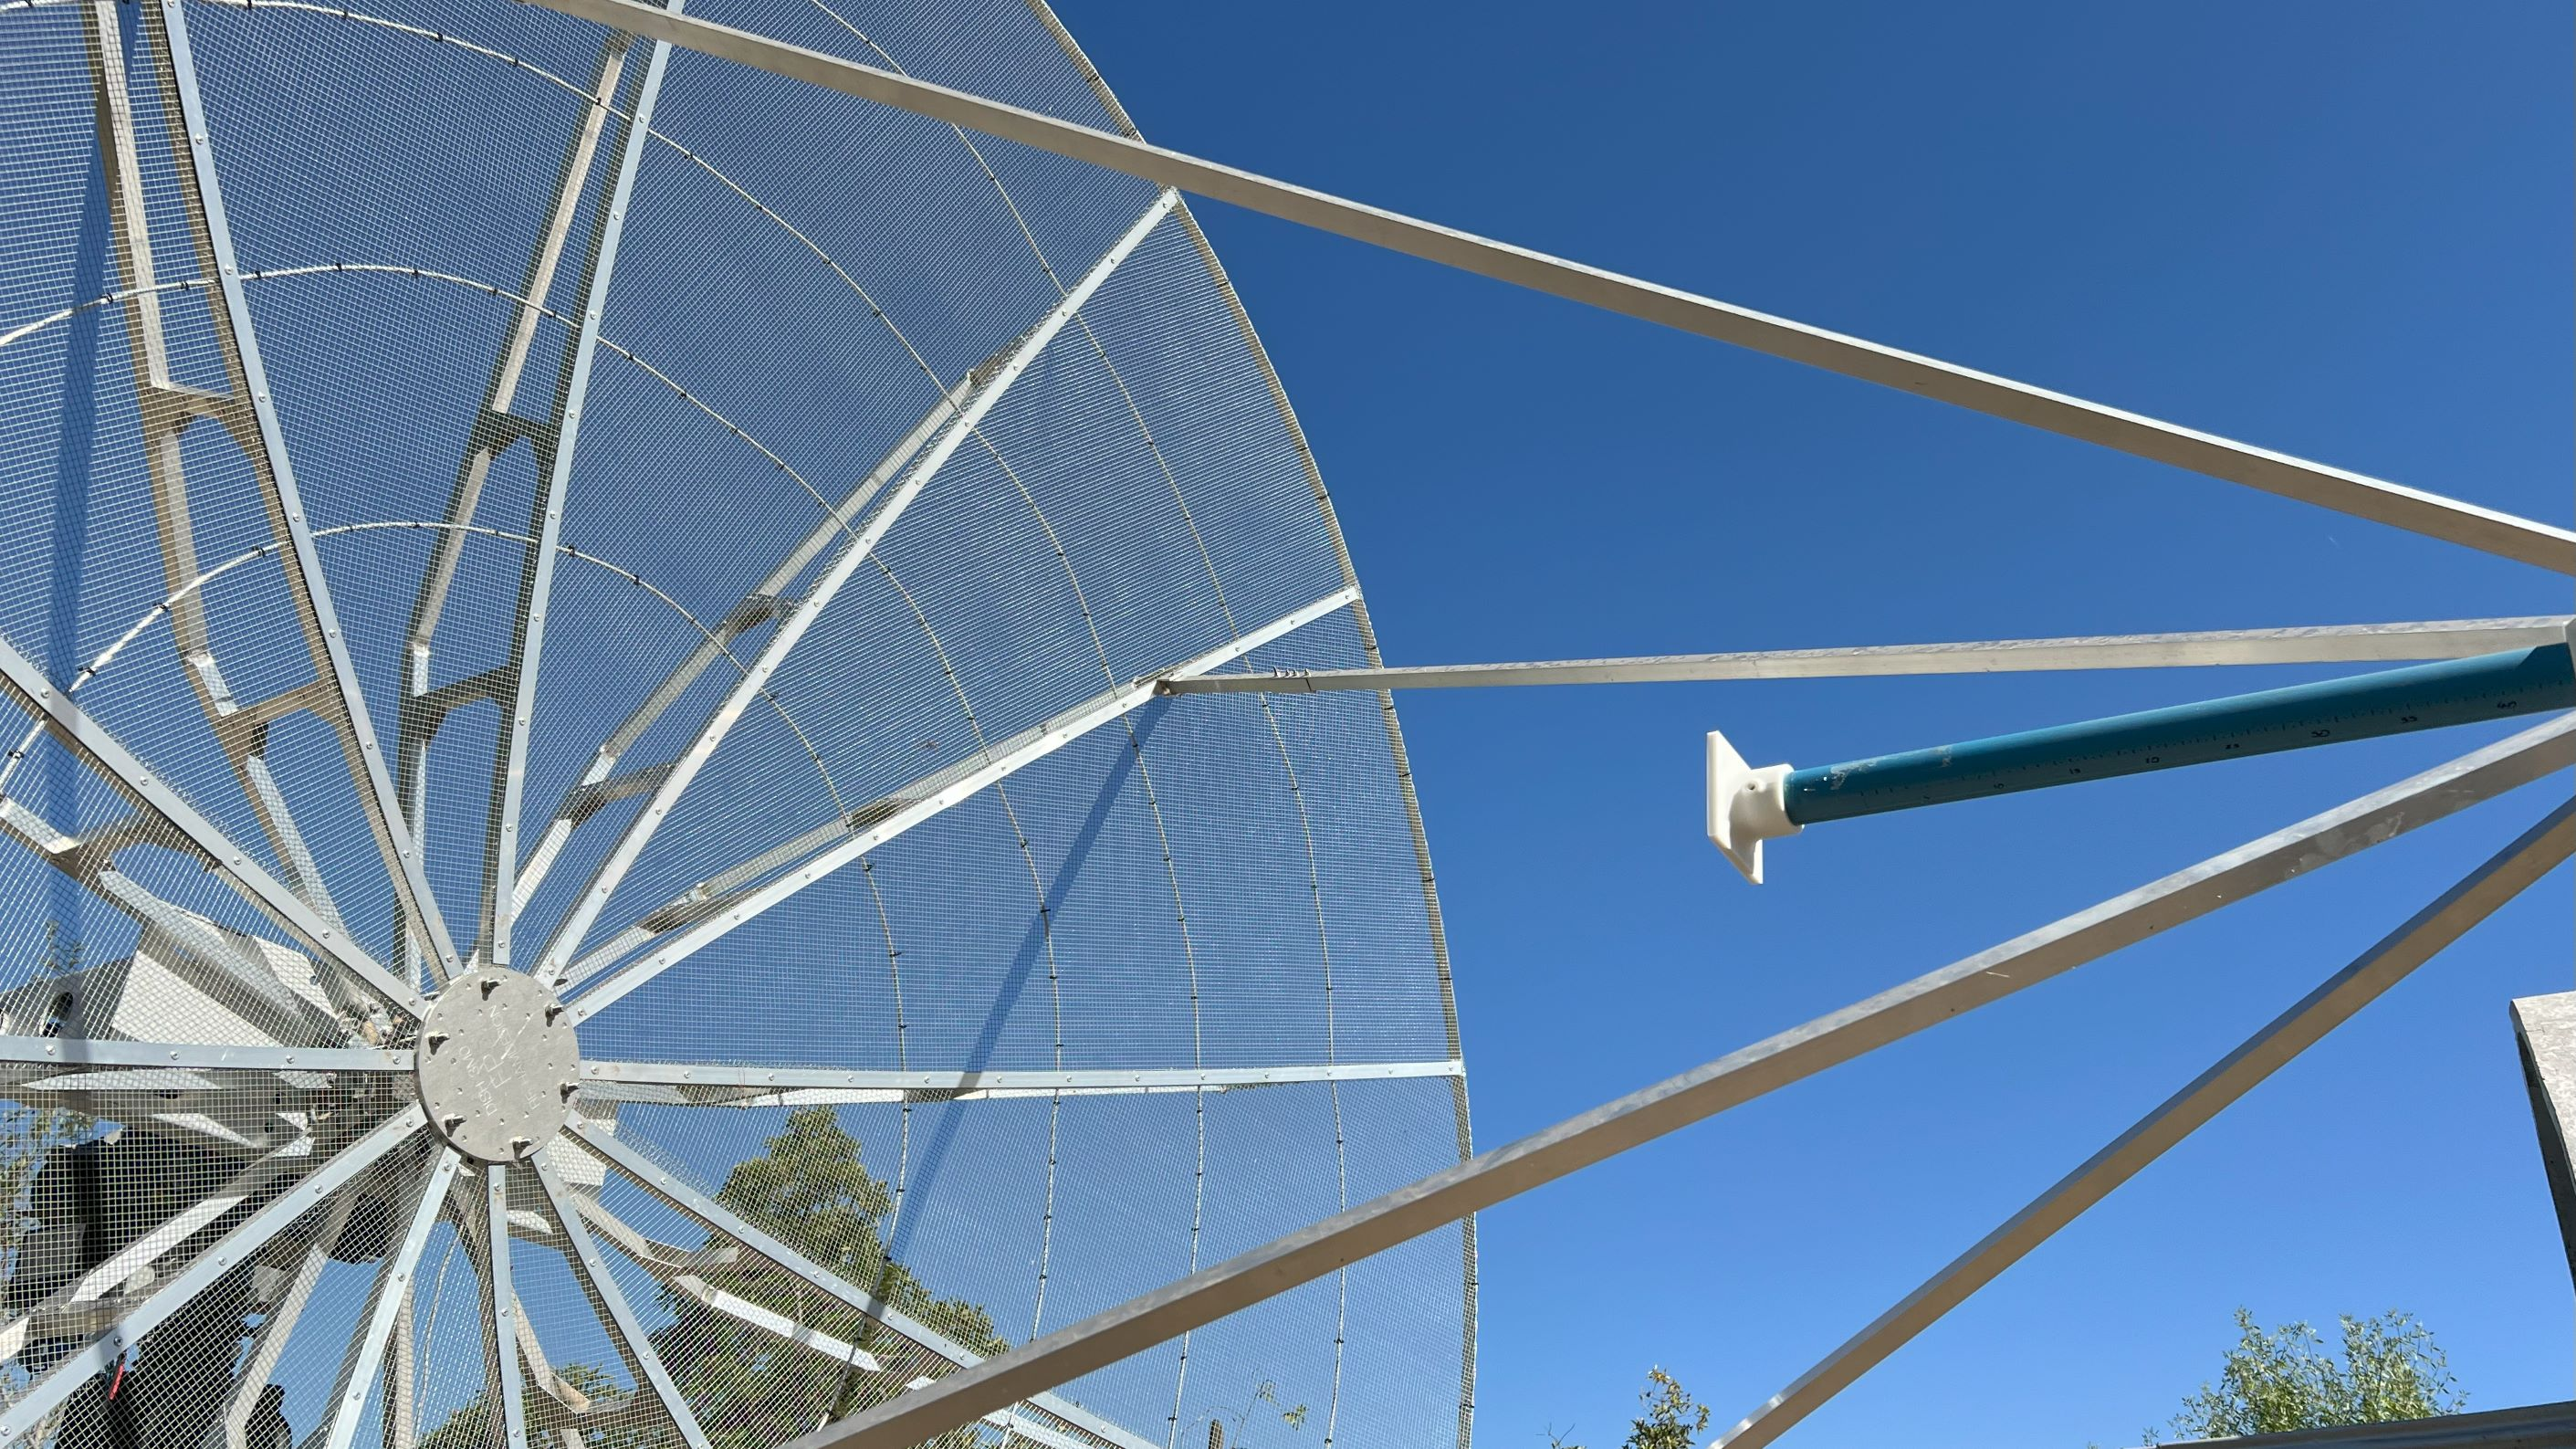
\includegraphics[width=0.7\textwidth]{img/feed_focus}
    \caption{Alimentador dipolo exotico con tetrapodo isntalado.}
    \label{fig:enfoque2}
\end{figure}

En la figura \ref{fig:enfoque2} se muestra el alimentador con el tetrapodo instalado y un tubo PVC milimetrado para medir la distancia relativa al reflector, usando de referencia el punto donde los soportes se unen al tubo del alimentador.\\

Para esta medicion de enfoque, se movio el alimentador en el eje Z con una resolucion de 0.5 cm hasta encontrar el punto de maxima potencia recibida. Se midio la razon señal a ruido y se obtuvo el punto de maxima potencia recibida en dBFS al igual que en la medicion anterior.\\

\section{Medicion del patrón de radiación}

Se utilizaron 2 plataformas para la medicion del patron de radiacion, una con la medida relativa dBFS obtenida de los espectros de la RTL-SDR y otra con la medida absoluta en dBm obtenida con el analizador de espectros Siglent SVA1075x. Para todas las mediciones se utilizó la estrella artificial de la copa de agua.\\

Todas las mediciones de patron de radiacion se realizaron en la cima del cerro Calan, en la plataforma de observacion del telescopio CPT. Para cada frecuencia medida, se hicieron los cortes azimutales y de elevecaion, o la medida del campo H y el campo E. Todos los cortes son de 180 grados para obtener con claridad los lobulos laterales y con una definicion de 1 punto por grado.\\


\subsection{Medicion relativa para banda de H1}

La medicion con la RTL-SDR se realizo a 1428MHz, utilizando el filtro angosto de la misma frecuencia de radioastronomy suplies. El generador Valon, se configuro a 1428MHz con una potencia inyectada a la estrella artificial de 0.23dBm.\\

Las perdidas ohmnicas del cable coaxial RG316 a 1428MHz son de 10.5 dB por 10 m, como el cable que alimenta la antena de la copa de agua es de 20 metros, se obtiene una perdida de 21 dB. La potencia recibida por la antena es de -21 dBm aproximadamente\\

Con los software de medicion se obtuvieron los espectros de la señal recibida por la RTL-SDR, se midio la razon señal a ruido y se guardaron 1000 espectros para cada grado de elevacion y azimut. Como la copa de agua se encuentra en altura, se genera un plano semicircular elevado en 7 grados sobre el eje horizontal, donde se corrigen los valores de elevacion por angulo azimutal con la ecuacion de correccion \ref{eq:powerdensity}. Para el segundo corte, se genera un ofset de 7 grados en elevacion, y para medir de 0 a -90 grados, se invierte la posicion azimutal en 180 grados para obtener ese cuadrante.\\

\subsection{Medicion absoluta para todas las badnas de interes}

\section{Sensibilidad y temperatura de ruido}

La medida de sensibilidad se realizó inyectando un tono para cada frecuencia de interes en la entrada de la cadena de recepcion. Se utilizó el generador de señales Rode and Schwartz SMB100A con una potencia de salida de -80 dBm y un coaxial RG316 de 10 metros al receptor instalado en el foco de la antena. Se midieron los espectros generados por la RTL-SDR para determinar la escala dBFS de la radio y calibrar los demás espectros en potencia.\\

Se guardaron los espectros de 300MHz, 400MHz y 500MHz para cubrir la banda de interes del proyecto CHARTS. Tambien se guardaron los espectros de 1000MHz, 1428MHz, 1500MHz y el límite de digitalizacion de 1700MHz.\\

\subsection{Medicion de la temperatura de ruido}

Para medir la temperatura de ruido y por ende la figura del receptor, se utilizó la fuente de ruido Agilent 346B con una amplificacion de 40dB. Para la cadena de amplificacion se utilizó el LNA + Filtro H1 SAWbird+ H1 de Nooelec, el cual se conectó a la fuente de ruido y se midio la potencia de ruido en la salida en el analizador de espectro.\\

Para la temperatura de ruido del receptor, se inyectó la señal de ruido en la entrada del receptor y se midio la potencia de ruido con los espectros de la RTL-SDR en la banda de interes.\\

Para obtener la temperatura del sistema completo se realizó una acumulacion de espectros del centro de la galaxia a 1420MHz y a una region del cielo limpia en concentracion de hidrógeno neutro. Consultando a los catalogos de radioastronomia se obtuvo la temperatura de la galaxia y de la region del cielo.\\

Con cada una de estas mediciones se realizó el cálculo de temperatura de ruido con el metodo de Y-factor y se obtuvo la figura de ruido de la cadena de amplificacion, del receptor y del sistema.\\


\section{Medicion del error de apuntamiento}

\section{Primera luz}

Para la primera luz, se escojio el centro de la galaxia por varias razones. La primera es que es una fuente de radio muy fuerte, facil de detectar y es bastamente estudiada y catalogada. La segunda razon es que para la epoca de medicion, noviembre, diciembre y enero, el centro de la galaxia se encuentra bastante cerca del cenit para la latitud de Santiago, lo que facilita la observacion.\\

El centro de la galaxia en una asencion recta de 17 h 45 m 40 s y una declinacion -29°00'28'', coordinendas que son ingresadas en el software de control de la montura alt azimutal. Se acumularon espectros por periodos de 2 horas por 3 dias, desde las 10 am hasta las 6 pm, para obtener la maxima cantidad de datos posibles. Tambien se descartaron algunas observaciones deonde el solo se encontraba muy cerca del centro de la galaxia, para evitar la saturacion del receptor.\\

Para la observacion se configuro el telescopio con el receptor de H1 y con la antena dipolo exotico en el foco geometrico del reflector. Se obtuvieron los espectros de la RTL-SDR y se guardaron en el disco duro para su posterior analisis.\\